
\documentclass[11pt, oneside]{book}

%%%%%%%%%%%%%%Include Packages%%%%%%%%%%%%%%%%%%%%%%%%%%
\usepackage{xcolor}
\usepackage{mathtools}
\usepackage[a4paper, total={6in, 8in}, margin=1.25in]{geometry}
\usepackage{amsmath}
\usepackage{amssymb}
\usepackage{paralist}
\usepackage{rsfso}
\usepackage{amsthm}
\usepackage{wasysym}
\usepackage[inline]{enumitem}   
\usepackage{hyperref}
\usepackage{tocloft}
\usepackage{wrapfig}
\usepackage{titlesec}
\usepackage{colortbl}
\usepackage{stackengine} 
\usepackage{listings}
%%%%%%%%%%%%%%%%%%%%%%%%%%%%%%%%%%%%%%%%%%%%%%%%%%%%%%%%



%%%%%%%%%%%%%%%Code%%%%%%%%%%%%%%%%%%%%%%%%%%%%%%%%%%%%%
\definecolor{codegreen}{rgb}{0,0.6,0}
\definecolor{codegray}{rgb}{0.5,0.5,0.5}
\definecolor{codepurple}{rgb}{0.58,0,0.82}
\definecolor{backcolour}{rgb}{0.95,0.95,0.92}

\lstdefinestyle{mystyle}{
    backgroundcolor=\color{backcolour},   
    commentstyle=\color{codegreen},
    keywordstyle=\color{magenta},
    numberstyle=\tiny\color{codegray},
    stringstyle=\color{codepurple},
    basicstyle=\ttfamily\footnotesize,
    breakatwhitespace=false,         
    breaklines=true,                 
    captionpos=b,                    
    keepspaces=true,                 
    numbers=left,                    
    numbersep=5pt,                  
    showspaces=false,                
    showstringspaces=false,
    showtabs=false,                  
    tabsize=2
}
%%%%%%%%%%%%%%%%%%%%%%%%%%%%%%%%%%%%%%%%%%%%%%%%%%%%%%%%

%%%%%%%%%%%%%%%Chapter Setting%%%%%%%%%%%%%%%%%%%%%%%%%%
\definecolor{gray75}{gray}{0.75}
\newcommand{\hsp}{\hspace{20pt}}
\titleformat{\chapter}[hang]{\Huge\bfseries}{\thechapter\hsp\textcolor{gray75}{$\mid$}\hsp}{0pt}{\Huge\bfseries}
%%%%%%%%%%%%%%%%%%%%%%%%%%%%%%%%%%%%%%%%%%%%%%%%%%%%%%%%

%%%%%%%%%%%%%%%%%Theorem environments%%%%%%%%%%%%%%%%%%%
\newtheoremstyle{break}
  {\topsep}{\topsep}%
  {\itshape}{}%
  {\bfseries}{}%
  {\newline}{}%
\theoremstyle{break}
\theoremstyle{break}
\newtheorem{axiom}{Axiom}
\newtheorem{thm}{Theorem}[section]
\renewcommand{\thethm}{\arabic{section}.\arabic{thm}}
\newtheorem{lem}{Lemma}[thm]
\newtheorem{cor}{Corollary}[thm]
\newtheorem{defn}{Definition}[thm]
\newenvironment{indEnv}[1][Proof]
  {\proof[#1]\leftskip=1cm\rightskip=1cm}
  {\endproof}
%%%%%%%%%%%%%%%%%%%%%%%%%%%%%%%%%%%%%%%%%%%%%%%%%%%%%%


%%%%%%%%%%%%%%%%%%%%%%%Integral%%%%%%%%%%%%%%%%%%%%%%%
\def\upint{\mathchoice%
    {\mkern13mu\overline{\vphantom{\intop}\mkern7mu}\mkern-20mu}%
    {\mkern7mu\overline{\vphantom{\intop}\mkern7mu}\mkern-14mu}%
    {\mkern7mu\overline{\vphantom{\intop}\mkern7mu}\mkern-14mu}%
    {\mkern7mu\overline{\vphantom{\intop}\mkern7mu}\mkern-14mu}%
  \int}
\def\lowint{\mkern3mu\underline{\vphantom{\intop}\mkern7mu}\mkern-10mu\int}
%%%%%%%%%%%%%%%%%%%%%%%%%%%%%%%%%%%%%%%%%%%%%%%%%%%%%%



\newcommand{\R}{\mathbb{R}}
\newcommand{\N}{\mathbb{N}}
\newcommand{\Z}{\mathbb{Z}}
\newcommand{\Q}{\mathbb{Q}}
\newcommand{\C}{\mathbb{C}}
\newcommand{\T}{\mathcal{T}}
\newcommand{\M}{\mathcal{M}}
\newcommand{\Symm}{\text{Symm}}
\newcommand{\Alt}{\text{Alt}}
\newcommand{\Int}{\text{Int}}
\newcommand{\Bd}{\text{Bd}}
\newcommand{\Power}{\mathcal{P}}
\newcommand{\ee}[1]{\cdot 10^{#1}}
\newcommand{\spa}{\text{span}}
\newcommand{\sgn}{\text{sgn}}
\newcommand{\degr}{\text{deg}}
\newcommand{\pd}{\partial}
\newcommand{\that}[1]{\widetilde{#1}}
\newcommand{\lr}[1]{\left(#1\right)}
\newcommand{\vmat}[1]{\begin{vmatrix} #1 \end{vmatrix}}
\newcommand{\bmat}[1]{\begin{bmatrix} #1 \end{bmatrix}}
\newcommand{\pmat}[1]{\begin{pmatrix} #1 \end{pmatrix}}
\newcommand{\rref}{\xrightarrow{\text{row\ reduce}}}
\newcommand{\txtarrow}[1]{\xrightarrow{\text{#1}}}
\newcommand\oast{\stackMath\mathbin{\stackinset{c}{0ex}{c}{0ex}{\ast}{\Circle}}}
\newcommand{\txt}{Wald's \textit{General Relativity}}

\newcommand{\note}{\color{red}Note: \color{black}}
\newcommand{\remark}{\color{blue}Remark: \color{black}}
\newcommand{\example}{\color{green}Example: \color{black}}
\newcommand{\exercise}{\color{green}Exercise: \color{black}}

%%%%%%%%%%%%%%%%%%%%%%Roman Number%%%%%%%%%%%%%%%%%%%%%%%
\makeatletter
\newcommand*{\rom}[1]{\expandafter\@slowromancap\romannumeral #1@}
\makeatother
%%%%%%%%%%%%%%%%%%%%%%%%%%%%%%%%%%%%%%%%%%%%%%%%%%%%%%%%%

%%%%%%%%%%%%%table of contents%%%%%%%%%%%%%%%%%%%%%%%%%%%%
%\setlength{\cftchapindent}{0em}
%\cftsetindents{section}{2em}{3em}
%
%\renewcommand\cfttoctitlefont{\hfill\huge\bfseries}
%\renewcommand\cftaftertoctitle{\hfill\mbox{}}
%
%\setcounter{tocdepth}{2}
%%%%%%%%%%%%%%%%%%%%%%%%%%%%%%%%%%%%%%%%%%%%%%%%%%%%%%%%%%


%%%%%%%%%%%%%%%%%%%%%Footnotes%%%%%%%%%%%%%%%%%%%%%%%%%%%
\newcommand\blfootnote[1]{%
  \begingroup
  \renewcommand\thefootnote{}\footnote{#1}%
  \addtocounter{footnote}{-1}%
  \endgroup
}
%%%%%%%%%%%%%%%%%%%%%%%%%%%%%%%%%%%%%%%%%%%%%%%%%%%%%%%%%

%%%%%%%%%%%%%%%%%%%%%Section%%%%%%%%%%%%%%%%%%%%%%%%%%%%%
\makeatletter
\def\@seccntformat#1{%
  \expandafter\ifx\csname c@#1\endcsname\c@section\else
  \csname the#1\endcsname\quad
  \fi}
\makeatother
%%%%%%%%%%%%%%%%%%%%%%%%%%%%%%%%%%%%%%%%%%%%%%%%%%%%%%%%%

%%%%%%%%%%%%%%%%%%%%%%%%%%%%%%%%%%%Enumerate%%%%%%%%%%%%%%
\makeatletter
% This command ignores the optional argument 
% for itemize and enumerate lists
\newcommand{\inlineitem}[1][]{%
\ifnum\enit@type=\tw@
    {\descriptionlabel{#1}}
  \hspace{\labelsep}%
\else
  \ifnum\enit@type=\z@
       \refstepcounter{\@listctr}\fi
    \quad\@itemlabel\hspace{\labelsep}%
\fi}
\makeatother
\parindent=0pt
%%%%%%%%%%%%%%%%%%%%%%%%%%%%%%%%%%%%%%%%%%%%%%%%%%%%%%%%%%



\begin{document}

	\begin{titlepage}
		\begin{center}
			\vspace*{0.5cm}
			\Huge \color{red}
				\textbf{Homework 9}\\
			\vspace{0.5cm}			
			\Large \color{black}
			Physics 542 - Quantum Optics\\
			Professor Alex Kuzmich
			\vspace{1.5cm}

			
\includegraphics[scale=1.15]{hmm.pdf}
			
			
			\vspace{2cm}
			\LARGE
				\textbf{Jinyan Miao}\\
				\hfill\break
				\LARGE Fall 2023\\
			\vspace{1cm}

		\vspace*{\fill}
		\end{center}			
	\end{titlepage}

\chapter{}
Here we consider 
\begin{align*}
S(N) = |A(N,t)|^2
\end{align*}
where we have
\begin{align*}
A(N,t) = \sum_{j=1}^N e^{-i \omega t + i \phi_j}
\end{align*}
with $\phi_j \in \R$ being random phase. Here we will compute, assume taking the time average,
\begin{align*}
\langle A\rangle = \left\langle e^{-i\omega t} \sum_{j=1}^N e^{i\phi_j}\right\rangle = 
0\cdot
\sum_{j=1}^N e^{i\phi_j} = 0\,.
\end{align*}
\begin{align*}
\langle S\rangle = 
\left\langle 
\sum_{j=1}^N e^{i\omega t -i\phi_j}
\sum_{k=1}^N e^{-i\omega t +i\phi_k}
\right\rangle =
\left\langle 
\sum_{j,k=1}^N e^{i(\phi_k-\phi_j)}\right\rangle = 
\sum_{j,k=1}^N e^{i(\phi_k-\phi_j)} = \sum_{j\leq k}^N 2\cos(\phi_j-\phi_k)\,.
\end{align*}
\begin{align*}
\langle
S^2
\rangle =  
\left\langle
\left( \sum_{j,k=1}^N e^{i(\phi_k -\phi_j)}\right)
\left( \sum_{j',k'=1}^N e^{i(\phi_{k'} -\phi_{j'})}\right)
\right\rangle= \left( \sum_{j\leq k}^N 2\cos(\phi_j-\phi_k) \right)\left( \sum_{j'\leq k'}^N 2\cos(\phi_{j'}-\phi_{k'})\right)\,.
\end{align*}
\begin{align*}
(\Delta S)^2 = \langle S^2\rangle - \langle S\rangle^2 = 0\,.
\end{align*}
Now compute, assuming taking the ensemble average (over $\phi_j$), 
\begin{align*}
\langle A\rangle = \left\langle e^{-i\omega t} \sum_{j=1}^N e^{i\phi_j}\right\rangle = 
 e^{-i\omega t}\cdot 0 = 0\,.
\end{align*}
\begin{align*}
\langle S\rangle = 
\left\langle 
\sum_{j=1}^N e^{i\omega t -i\phi_j}
\sum_{k=1}^N e^{-i\omega t +i\phi_k}
\right\rangle =
\left\langle 
\sum_{j,k=1}^N e^{i(\phi_k-\phi_j)}\right\rangle = N\,.
\end{align*}
\begin{align*}
\langle
S^2
\rangle =  
\left\langle
\left( \sum_{j,k=1}^N e^{i(\phi_k -\phi_j)}\right)
\left( \sum_{j',k'=1}^N e^{i(\phi_{k'} -\phi_{j'})}\right)
\right\rangle =
\left\langle 
\sum_{j,k,j',k' = 1}^N e^{i(\phi_k -\phi_j+\phi_{k'}-\phi_{j'})}
\right\rangle = 2N^2 - N\,.
\end{align*}
\begin{align*}
(\Delta S)^2 = \langle S^2\rangle - \langle S\rangle^2 = 2(N^2 - N)\,.
\end{align*}
Quantities are computed with the help of Eq.\,(13.61) and (13.64) on Berman's text. 

\chapter{}
We evaluate 
\begin{align*}
S = \left|\sum_{j=1}^{100} e^{-i\omega t+ i\phi_j} \right|
\end{align*}
with random phases $\phi_j$ picked via random number generator. The three $S$'s that we obtain are $S = 3.59$, $S=114.65$, and $S=94.02$. Then we repeat the calculation of $S$ for a $1000$ times and take the average, $\langle S\rangle = 98.18$ in this case, the result is shown on next page.
\newpage
\begin{center}
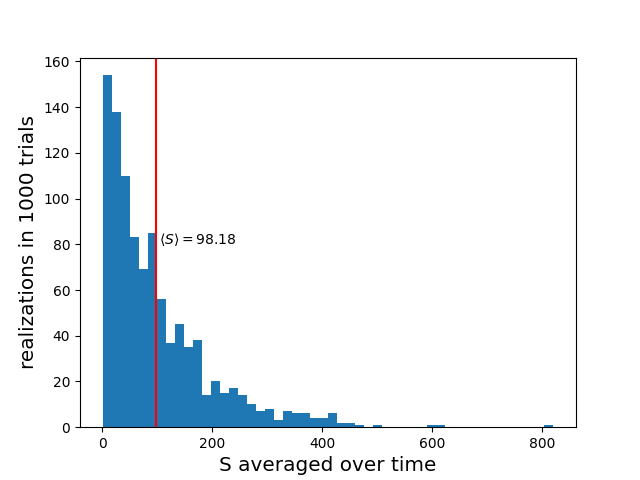
\includegraphics[scale=0.65]{542HW9/P2}
\end{center}
We do the same thing for $S^2$.
\begin{center}
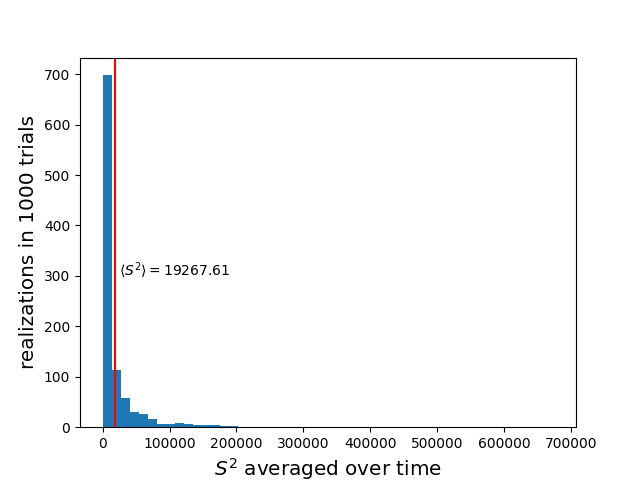
\includegraphics[scale=0.65]{542HW9/P2S2}
\end{center}
\newpage
Now we evaluate them 100000 times, the numbers that we get here are very close to what we have calculated in problem 1. 
\begin{center}
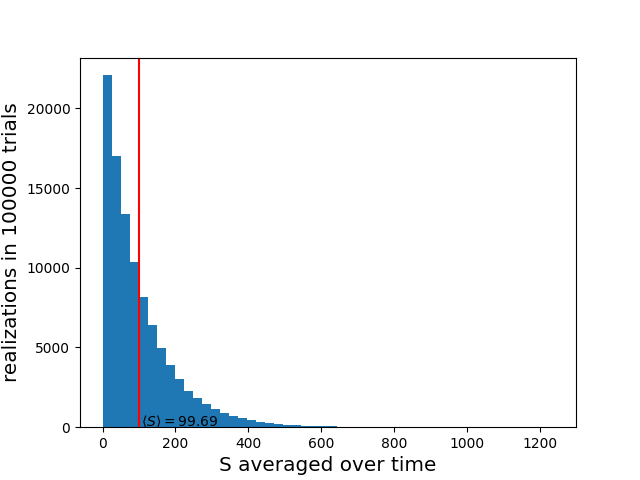
\includegraphics[scale=0.65]{542HW9/P2More}
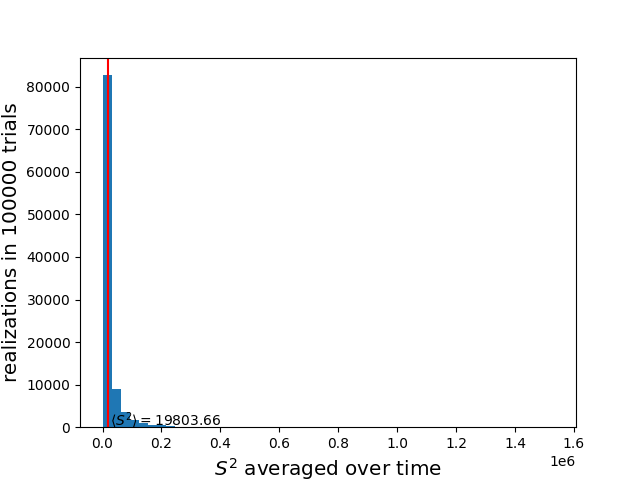
\includegraphics[scale=0.65]{542HW9/P2S2More}
\end{center}

\chapter{}
First we consider 
\begin{align*}
I(t) = \sum_{n=-\infty}^\infty \Theta(t+0.1-n) -\Theta(t-0.1-n)
\end{align*}
where $\Theta$ is the Heaviside step function. It is not hard to see that 
\begin{align*}
\bar{I} = 
\lim_{T\to \infty}\frac{1}{T}\int_{-T/2}^{T/2}I(t) \, dt
=
\lim_{T\to \infty}\frac{1}{T} \left(\lfloor T\rfloor \cdot 0.2 + \mu\right)= 0.2\,,
\end{align*} 
where $|\mu| <1$.  To compute $\langle I(t) \, I(t+\tau)\rangle$, as $I$ is periodic with periods $1$, it is not hard to see that $\langle I(t+n)\,I(t)\rangle = 0.2$ for all $n\in \N$ by symmetry. Furthermore, for $0.2\leq \tau \leq 0.8$, we have either (1) $I(t+\tau) = 0$ with $I(t) =1$, or (2) $I(t+\tau) = 1$ with $I(t) = 0$, thus their product must be $\langle I(t) \, I(t+\tau) \rangle = 0$ when $0.2\leq \tau \leq 0.8$. Lastly, for $0< \tau < 0.2$, by the periodicity of $I$, it is not hard to see that the time average of the product $\langle I(t) \, I(t+\tau) \rangle = 0$ decreases linearly from $0.2$ to $0$ as a function of $\tau$. Then using periodicity and symmetry, we conclude 
\begin{align*}
g^{(2)}(\tau) = \begin{cases}
1- 5 \cdot |\tau -\text{round}(\tau)| & |\tau -\text{round}(\tau)| \leq 0.2 \\
0 & |\tau -\text{round}(\tau)|> 0.2
\end{cases} \,, \tag{*}
\end{align*}
where round$(\cdot)$ is the function that rounds to the nearest integer. We calculate $g^{(2)}$ from the definition using $I$, and compare that with the result we obtain in Eq.\,(*). 

\begin{center}
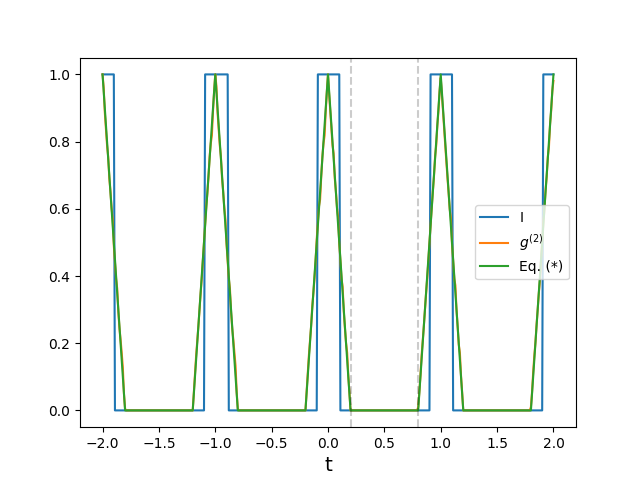
\includegraphics[scale=0.65]{542HW9/P3}
\end{center}
The gray dashed lines are $t = 0.2$ and $t = 0.8$, respectively. Here $g^{(2)}(\tau)$ does not approach $0$ as $\tau \to \infty$ as $I$ is a periodic function of time, which implies $I(t)$ and $I(t+\tau)$ are for sure correlated. 
 
\newpage
Here we consider
\begin{align*}
E^+(t) = \frac{e^{-i\omega t}}{\pi^{1/4}}e^{-t^2/2}\,.
\end{align*}
Thus we can compute
\begin{align*}
E^-(t) = (E^+)^* = \frac{e^{i\omega t}}{\pi^{1/4}}e^{-t^2/2}\,,
\end{align*}
then we have
\begin{align*}
g^{(1)}(\tau) = \frac{\langle E^-(t)\, E^+(t+\tau)\rangle}{\langle E^-(t)\, E^+(t)\rangle} 
&= 
\frac{\lim_{T\to \infty}\frac{1}{T \pi^{1/2}}\int^{T/2}_{-T/2} e^{-(t^2+(t+\tau)^2))/2}e^{-i\omega\tau}\, dt}{\lim_{T\to \infty}\frac{1}{T\pi^{1/2}}\int^{T/2}_{-T/2}e^{-t^2}\,dt}\\
&=\frac{e^{-i\omega\tau}\lim_{T\to \infty}\int^{T/2}_{-T/2} e^{-(t^2+(t+\tau)^2))/2}\, dt}{\lim_{T\to \infty}\int^{T/2}_{-T/2}e^{-t^2}\,dt}\\
&=\frac{e^{-i\omega\tau}}{\pi^{1/2}} \lim_{T\to \infty}\int^{T/2}_{-T/2} e^{-(t^2+(t+\tau)^2))/2}\, dt\\
&= e^{-i\omega \tau - \tau^2/4}\,.
\end{align*}
While on the other hand,
\begin{align*}
g^{(2)}(\tau) &= \frac{\langle E^-(t)\,E^-(t+\tau) \,E^+(t+\tau)\, E^+(t)\rangle}{\langle E^-(t) \, E^+(t)\rangle^2}\\
&= \frac{\langle
e^{i\omega t-t^2/2}
e^{i\omega(t+\tau)-(t+\tau)^2/2}
e^{-i\omega t-t^2/2}
e^{-i\omega(t+\tau)-(t+\tau)^2/2}
 \rangle}{\langle
e^{-t^2}
\rangle^2}\\
%= e^{-\tau^2}\frac{\langle
%e^{-2t^2-2\tau t}
% \rangle}{\langle
%e^{-t^2}
%\rangle^2}\\
&= e^{-\tau^2}\frac{\lim_{T\to \infty}\frac{1}{T} \int_{-T/2}^{T/2} 
e^{-2t^2-2\tau t}\, dt
}{\lim_{T\to \infty}\frac{\pi}{T^2}
}\\
&= \frac{\pi^{1/2}e^{\tau^2/2}e^{-\tau^2}}{ 2^{1/2} \pi}\frac{\lim_{T\to \infty}\frac{1}{T} 
}{\lim_{T\to \infty}\frac{1}{T^2}
}\\
&= \frac{e^{-\tau^2/2}}{ (2\pi)^{1/2}}\lim_{T\to \infty} T
\end{align*}
which is an ill-defined quantity and obviously $g^{(2)}(0) = \infty$. 


\chapter{}
\begin{center}
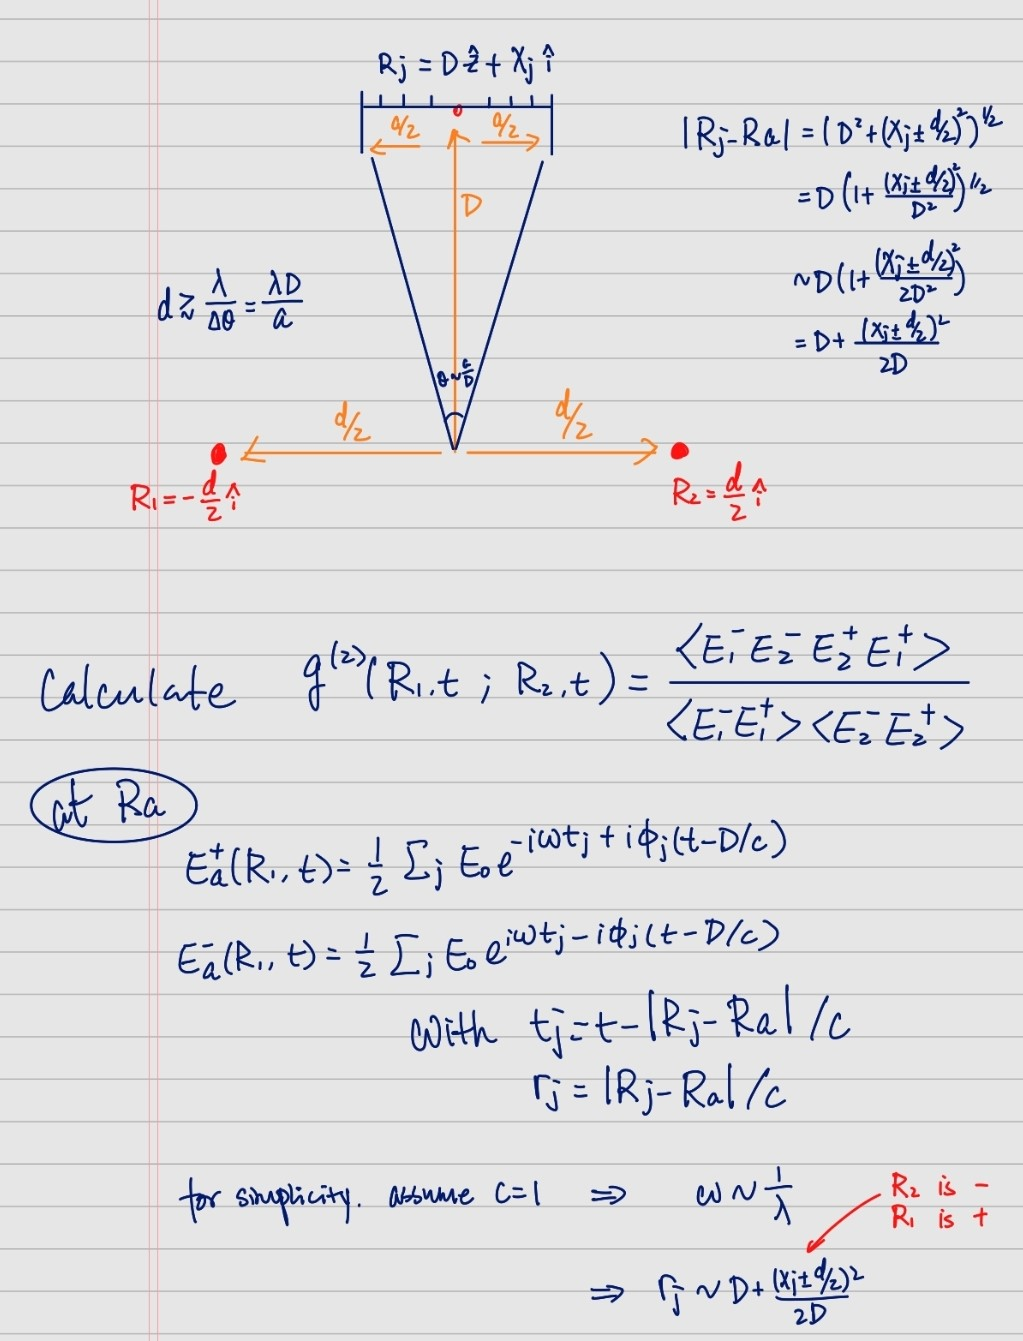
\includegraphics[scale=0.5]{542HW9/P42}
\newpage
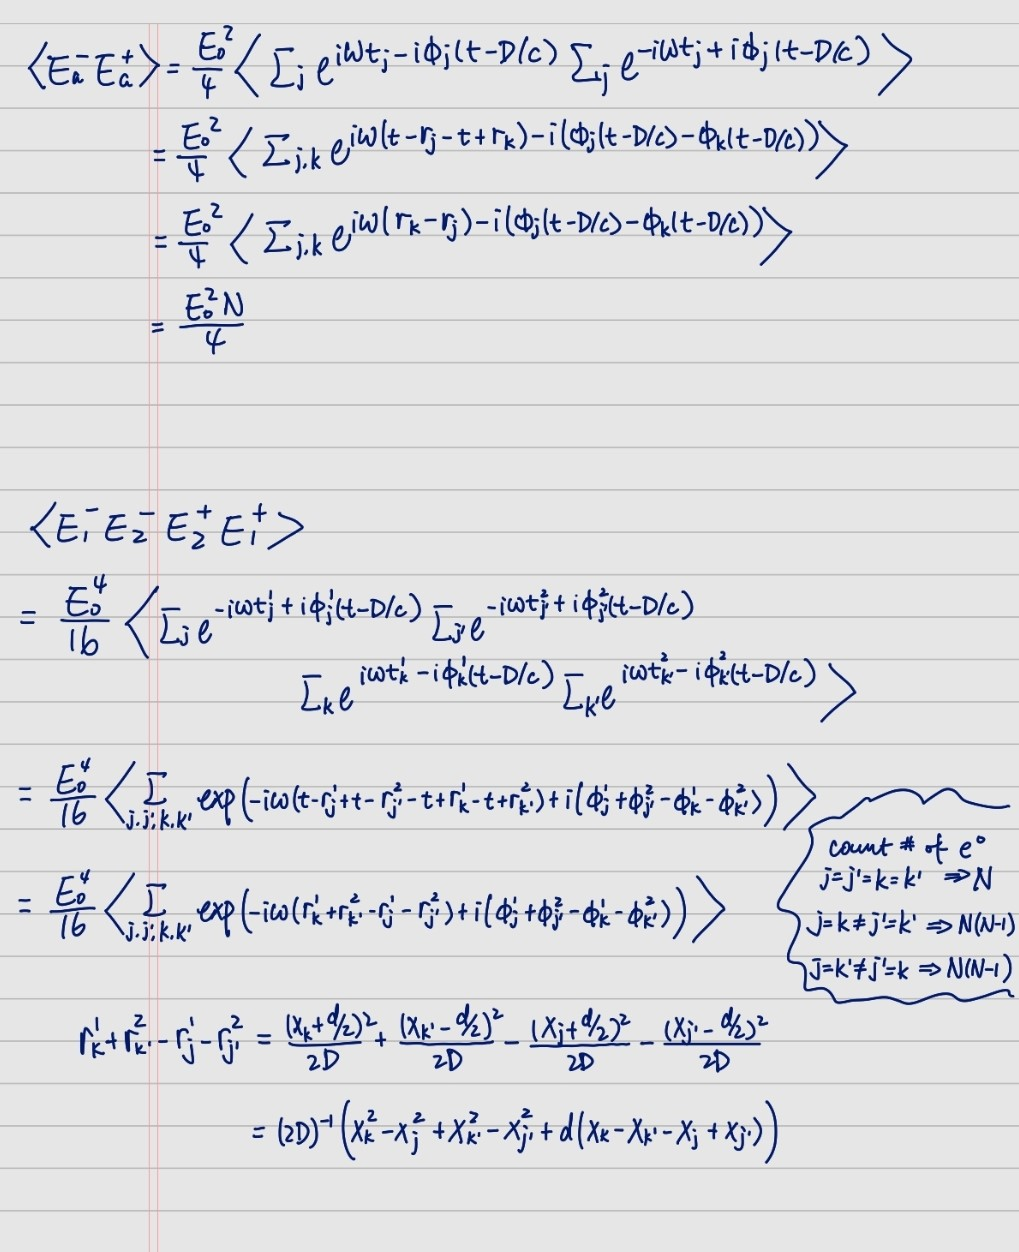
\includegraphics[scale=0.5]{542HW9/P41}
\end{center}



\end{document}



